\documentclass[12pt,letterpaper]{hmcpset}
\usepackage[margin=1in]{geometry}
\usepackage{graphicx}
\usepackage{amsmath}

% info for header block in upper right hand corner
\name{ }
\class{Math 172}
\assignment{Assignment 4}
\duedate{Tuesday, February 20, 2018}

\newcommand{\pn}[1]{\left( #1 \right)}
\newcommand{\abs}[1]{\left| #1 \right|}
\newcommand{\bk}[1]{\left[ #1 \right]}

\newcommand{\vb}{\mathbf{v}}
\newcommand{\ub}{\mathbf{u}}
\newcommand{\fx}{f \left( x \right) =}
\newcommand*\LH{\ensuremath{\overset{\kern2pt L'H}{=}}}
\renewcommand{\labelenumi}{{(\alph{enumi})}}

\newcommand{\Ff}{\mathbb{F}}
\newcommand{\Zz}{\mathbb{Z}}
\newcommand{\Rr}{\mathbb{R}}
\newcommand{\Qq}{\mathbb{Q}}
\newcommand{\Cc}{\mathbb{C}}

\begin{document}

\problemlist{13.2 ( 4, 12, 14 ) 13.3 ( 1, R2 ) 13.4 ( 2, 3, R4 )}

\begin{problem}[13.2.4]
  Determine the degree over $\Qq$ of $2+\sqrt{3}$ and of $1 + \sqrt[3]{2} + \sqrt[3]{4}.$
\end{problem}
\begin{solution}
\vfill
\end{solution}
\newpage

\begin{problem}[13.2.12]
  Suppose the degree of the extension $K/F$ is a prime $p$. Show that any subfield $E$ of $K$ containing $F$ is either $K$ or $F$.
\end{problem}
\begin{solution}
	\vfill
\end{solution}
\newpage

\begin{problem}[13.2.14]
  Prove that if $[F(\alpha) : F]$ is odd then $F(\alpha) = F(\alpha^2).$
\end{problem}
\begin{solution}
	\vfill
\end{solution}
\newpage

\begin{problem}[13.3.1]
	Prove that it is impossible to construct the regular 9-gon.
\end{problem}
\begin{solution}
	\vfill
\end{solution}
\newpage

\begin{problem}[READ ONLY 13.3.2]
	Prove that Archimedes' construction actually trisects the angle $\theta$. [Note the isosceles triangles in Figure 5 to prove that $\beta = \gamma = 2\alpha$.]
	\begin{center}
		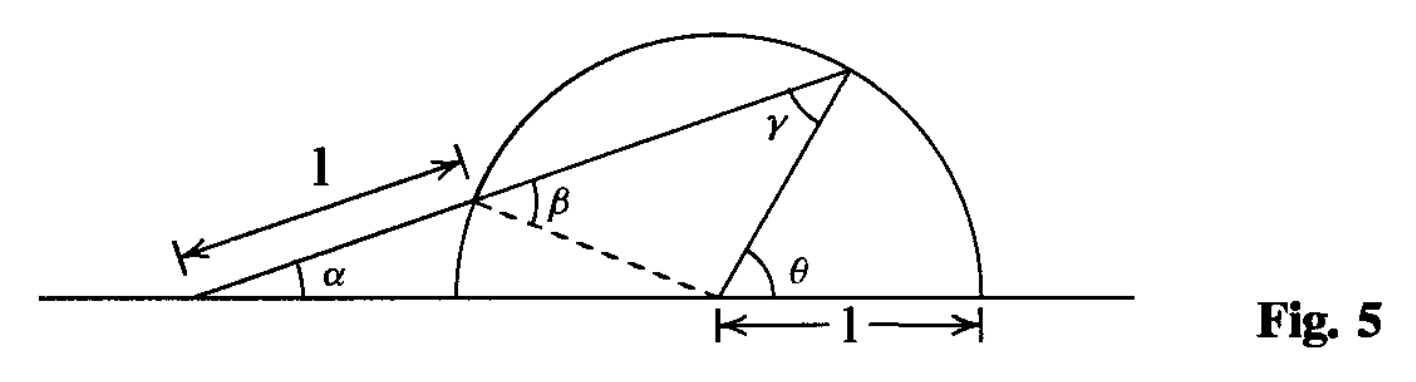
\includegraphics[scale=0.5]{13-3fig5.png}
	\end{center}
\end{problem}

\begin{problem}[13.4.2]
	Determine the splitting field and its degree over $\Qq$ for $x^4 + 2$.
\end{problem}
\begin{solution}
	\vfill
\end{solution}
\newpage

\begin{problem}[13.4.3]
	Determine the splitting field and its degree over $\Qq$ for $x^4 + x^2 + 1$.
\end{problem}
\begin{solution}
	\vfill
\end{solution}
\newpage

\begin{problem}[READ ONLY 13.4.4]
	Determine the splitting field and its degree over $\Qq$ for $x^6 - 4$.
\end{problem}
\end{document}
